\documentclass[12pt]{article}
\usepackage{amsmath, amsthm}
\usepackage[pdftex]{graphicx}
\usepackage{psfrag,epsf}
\usepackage{enumerate}
\usepackage{natbib}
\usepackage{float}
\restylefloat{table}

\usepackage{amssymb}
\usepackage{multirow}
\usepackage{float}
\newtheorem{thm}{Theorem}

\newcommand{\blind}{0}

\addtolength{\oddsidemargin}{-.75in}%
\addtolength{\evensidemargin}{-.75in}%
\addtolength{\textwidth}{1.5in}%
\addtolength{\textheight}{1.3in}%
\addtolength{\topmargin}{-.8in}%

\newtheorem{theorem}{\bf Theorem}
\newtheorem{proposition}{\bf Proposition}
\newtheorem{lemma}{\bf Lemma}
\newtheorem{corollary}{\bf Corollary}
\numberwithin{equation}{section}

\date{\textbf{Draft} \textbf{\today}}
\begin{document}

%\bibliographystyle{natbib}

%\newcommand{\keywords}[1]{\par\addvspace\baselineskip
%\noindent\keywordname\enspace\ignorespaces#1}

\def\spacingset#1{\renewcommand{\baselinestretch}%
{#1}\small\normalsize} \spacingset{1}


%%%%%%%%%%%%%%%%%%%%%%%%%%%%%%%%%%%%%%%%%%%%%%%%%%%%%%%%%%%%%%%%%%%%%%%%%%%%%%

\if0\blind
{
  \title{Computing the Log Concave NPMLE for Interval Censored Data}
  \author{Clifford Anderson-Bergman\\
    Department of Statistics, University of California, Irvine\\
      Yaming Yu\\
    Department of Statistics, University of California, Irvine\\
    }
  \maketitle
} \fi

\if1\blind
{
  \bigskip
  \bigskip
  \bigskip
  \begin{center}
    {\LARGE\bf Computing the Log Concave NPMLE for Interval Censored Data}
\end{center}
  \medskip
} \fi


\spacingset{1.45}


\begin{abstract}

	In analyzing interval censored data, a non-parametric estimator is often desired, in part due to difficulties in assessing model fits. Much work has been put into the computation of the non-parametric maximum likelihood estimator (NPMLE). However, the estimates for values of interest of the survival function, such as the quantiles, have very large standard errors due to the jagged form of the estimator. In addition, the density and hazard functions are undefined by the estimator. By forcing the estimator to be constrained to the class of log concave functions, we insure a once differentiable survival estimator which has much better operating characteristics than the unconstrained NPMLE and specified density and hazard estimates. In this paper, we develop an effective algorithm for computing the log concave NPMLE. Using simulated data, we show that this new estimator has favorable operating characteristics compared to the unconstrained NPMLE and another competing modern estimator for interval censored data. We illustrate our method with current status data for the onset of menopause. 
\end{abstract}

 {\bf Keywords}: Shape Constraints, Log Concave, Interval Censored, Active Set Algorithm

{\section{Introduction}}

	Interval censoring occurs when the time to event is known only up to an interval, \emph{i.e.} the $i^{th}$ event time is only known to have occurred after $L_{i}$ and before $R_i$. A special case of interval censoring that we will examine is {\it case I} interval censored data, or current status data. In this case, each subject $i$ is inspected at a random time $C_i$. The only information collected is whether the event of interest has occurred before $C_i$ (in which case $L_i$ = 0 and $R_i$ = $C_i$) or the event has not occurred by time $C_i$ (in which case $L_i$ = $C_i$ and $R_i$ = $\infty$). Thus, for case I interval censoring all the data is either left or right censored. In the case of {\it case II} interval censoring, the data can be left censored, right censored or known up to an interval (i.e. $L_i > 0$ and $R_i < \infty$). 
	
	For such data, model assessment can be very difficult, as visual plots such as histograms cannot be used. As a result, there is high demand for non parametric estimators, which tend to rely less heavily on model assumptions. The non-parametric maximum likelihood estimator (NPMLE) has been studied in depth (Turnbull 1976, Gentleman and Geyer 1994, Huan and Wellner 1997, Jongbloed 1998) and is often the estimator of choice. This will be referred to as the unconstrained NPMLE for the remainder of this article. The unconstrained NPMLE is known to be consistent for the survival distribution in the univariate case (Gentleman and Geyer 1994). However, for any finite sample size, the estimator shows erratic jumps (see figure 1), making any density estimate degenerate and resulting in high variance of the estimated quantiles. 
	
\begin{figure}[h]
\centerline{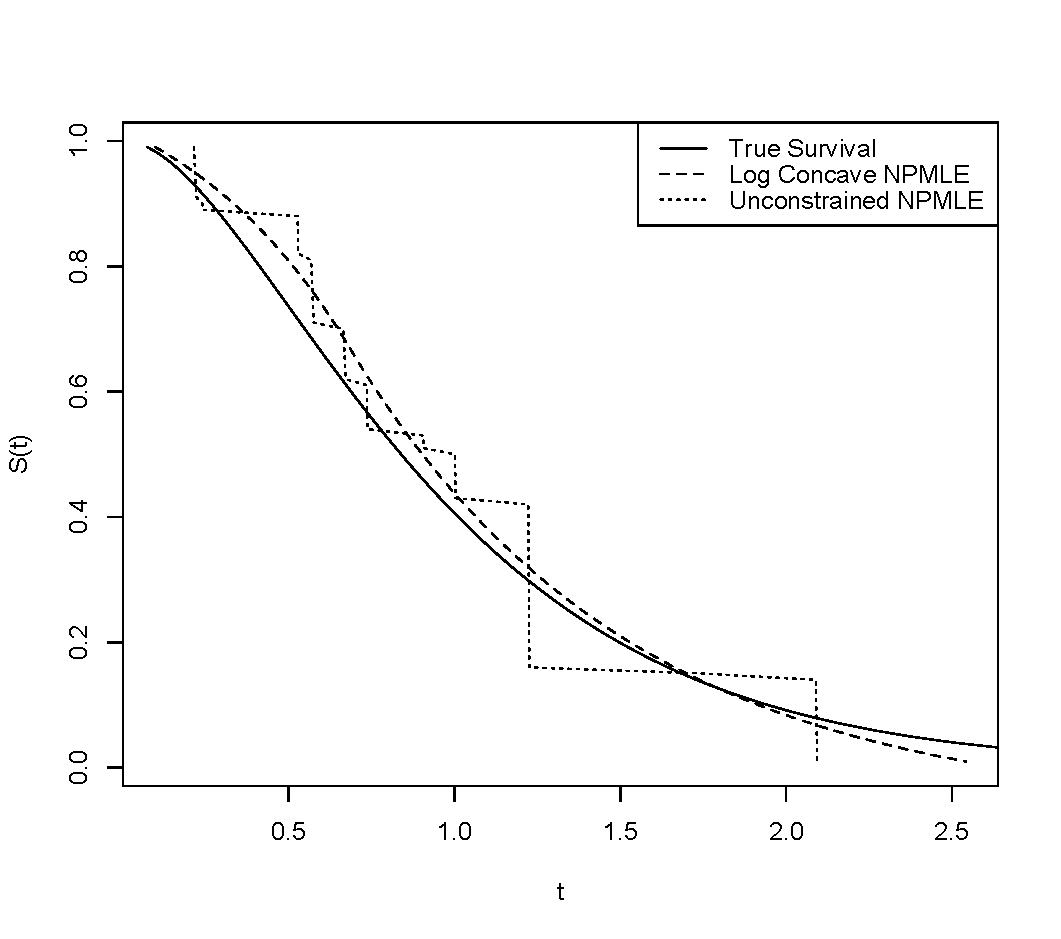
\includegraphics[width = 9cm]{LCvUC.pdf} }
\caption{Log concave NPMLE and unconstrained NPMLE. Data are current status data simulated from a Gamma(2,2) distribution with $n = 400$ }
\end{figure} 
			
	There are several approaches to a smoothing the estimator in order to improve operating characteristics. One is smoothing over the unconstrained NPMLE with a kernel estimator (Betensky et al 1999). Another technique is to model the density with log-spline functions, using AIC to select the number of knots (Kooperberg and Stone, 1992). While both of these techniques have been shown to reduce the variance of the estimated survival curve for interval censored data (Pan 2000), they have their drawbacks as well. Both these estimators require selecting some form of smoothing parameter, which can be non-trivial in the interval censored case. As an example, the log spline density estimator can be found in the CRAN package  ``logspline", with preset smoothing penalties. While this estimator can preform well with light censoring, in our experience with simulated data, it behaves poorly under heavy censoring. In particular, it was often observed that either the estimate of the density jumps highly erratically or the algorithm fails to converge when used with current status data, even for large data sets (in fact, the estimator appears to preform \emph{worse} for larger data sets). Similar problems were noted in Pan 2000.  Likewise, the question of bandwidth selection for the kernel smoother for interval censored data is still an open question. In this study, we find that the current bandwidth selection methods can lead to heavy biases in quantile estimation. This produces demand for a fully automated, theoretically justified smooth estimator.
	
	Many researchers have investigated using various smoothness assumptions (rather than smoothness parameters) to improve the operating characteristics of the estimator. An early example of such an estimate is that of a non-increasing density (Grenander 1956). An extension of the non-increasing density is the uni-modal density (non-decreasing before the mode, non-increasing after), but the uni-modal NPMLE has been shown to be inconsistent at the mode (Wegman 1969). Another popular shape constraint is that of log concavity (Bagnoli and Bergstorm 2005). This assumption is considered very flexible as many parametric distributions fit into this category. The families of log concave distributions include normal, gamma with shape parameter $\ge$ 1, all Weibull densities with exponent $\ge$ 1, all beta densities with both parameters $\ge$ 1 and the logistic density. Non-logconcave distributions include the t-distribution, the lognormal distribution and any multimodal distribution. However, the log concave estimator has been shown to be useful in mixture modeling (Chang and Walther 2007) so it can be useful for multimodal data as well. This estimator is a consistent estimator of the density in the case of exact data (D\"umbgen and Rufibach 2009) and an efficient algorithm for finding the log concave NPMLE has been written for exact data (Rufibach 2007). 
		
	The problem is much more difficult for interval censored data. At the same time, there is more utility in a log concave estimator for interval censored data than in the case of exact data. By forcing the estimated density to be log concave, a fairly flexible assumption, one can greatly improve the operating characteristics of the estimated survival function without having to make more limiting assumptions of families of parametric distributions which can be very difficult to assess for interval censored data. However, computing the NPMLE is challenging for this case. Currently, there is an EM algorithm which requires discretizing the data and thus estimates an approximation (D\"umbgen et al 2011). In this paper, we aim at an exact solution without discretization.  We first prove a theorem that reduces the number of parameters required to characterize the log concave NPMLE to a finite set.  Even with a finite support set, however, log-likelihood functions involving interval censored data often are not strictly concave, making maximization very difficult (the reader must be very careful to note the distinction between the log likelihood being concave and the estimator being log concave). Therefore one of our main contributions is an algorithm for finding a log concave NPMLE solution over those parameters. It is worth noting that the algorithm presented in this paper is considerably faster than the discrete approximation in its current form. For a sample of size $n = 25$, the discrete approximation took on average 12 seconds, whereas the algorithm we present took on average 0.05 seconds. For $n = 50$, the discrete approximation took 31 seconds, while ours took 0.11. (Simulations were done in R, using a Macbook with a 2GHz Intel Core 2 Duo processor with 4 GB of RAM. Our algorithm was written in R, using the Rcpp package to create C++ functions for the likelihood and derivative functions. Their algorithm was provided in the CRAN package ``logconcens".) Solutions were visually identical. Average times for our algorithm for larger data sets is presented in section 10.2.1 in the appendix.
	
	The rest of this paper is organized as follows.  In Section~2, we formulate the likelihood function that we are interested in maximizing. In Section~3, we prove a theorem which shows that the maximum likelihood can be achieved by a function of a finite number of parameters. In Section~4, we present the different parameterizations that will be used in the algorithm. In Section~5, we discuss the convergence criterion, which is a crucial part of our proposed algorithm. In Section~6, we describe the algorithm itself. In Section~7, we apply the algorithm to a classic sample data set and compare the results to those of the unconstrained NPMLE and the kernel smoother. In Section~8, we simulate data and compare the bias and standard deviations of the log concave NPMLE, the unconstrained NPMLE and the kernel smoother across several different simulation scenarios. In Section~9, we discuss future research topics for the log concave NPMLE.
	 
	 
{\section {Likelihood Function}}


	For the $i^{th}$ subject, suppose the exact event time is known to be within the observation interval $[L_i, R_i]$.  We adopt the standard assumption of independent observations among subjects and an independent censoring mechanism. Let $\phi(x)$ represent the log density at time $x$.  Then the log concave NPMLE is 
	
	\[ \hat \phi(x) =\underset{\phi(x)} {\arg \max} \displaystyle \sum_{i = 1}^n \log \left( \int_{L_i}^{R_i} e^ { \phi(x) } \,dx \right)
	\]
	\[
	 s.t.\quad \frac{ \phi(x_2) - \phi(x_1)} {x_2 - x_1} \geq \frac{ \phi(x_3) - \phi(x_2)} {x_3 - x_2} \quad \forall x_1 < x_2 < x_3 
	 \]
	 \[ \int_{-\infty}^{\infty} e^{\phi (x) } \,dx = 1
		\]

	To ease the last restriction, we replace $e^{\phi(x)}$ with $\frac{e^{\phi(x)} } { \int  e^{\phi(x)} dx}$, so that $e^{\hat \phi(x)}$ is proportional to the LC NPMLE. Under this parameterization, the LC NPMLE is written as 

	\[ \hat \phi(x) = \underset{\phi(x)} {\arg \max} \displaystyle \sum_{i = 1}^n \log \left( \int_{L_i}^{R_i} e^ { \phi(x) } \,dx \right) - n \times \log \left(  \int_{-\infty}^{\infty} e^ { \phi(x) } \,dx \right) 
	\]
	\[
	 s.t.\quad \frac{ \phi(x_2) - \phi(x_1)} {x_2 - x_1} \geq \frac{ \phi(x_3) - \phi(x_2)} {x_3 - x_2}\quad \forall x_1 < x_2 < x_3 
	 \]
	
	Note that under this parameterization, $\hat \phi(x)$ is calculated up to an additive constant. For simplicity we set $\max_x $ $\hat \phi(x) = 0$. We can then interpret $\hat \phi(x)$ as the estimated log ratio between the density at $x$ and the density at the mode.

	The log-concave restrictions ensure that $\phi(x)$ is continuous on the closed interval for which $e^{\phi(x)} > 0$ (i.e., the support of the density), and both its left and right derivatives exist in the interior of the support. It follows that the estimated survival function will be continuously once differentiable on the support of the density.
	
	In contrast, the unconstrained NPMLE is defined as 

	\[ \hat \phi(x) =\underset{\phi(x)} {\arg \max} \displaystyle \sum_{i = 1}^n \log \left( \int_{L_i}^{R_i} e^ { \phi(x) } \,dx \right)
	\]
	 \[ \int_{-\infty}^{\infty} e^{\phi (x) } \,dx = 1
		\]
	
	It has been shown that the solution to the unconstrained NPMLE only assigns mass to certain intervals called Turnbull intervals (Turnbull 1976) or maximal intersections. How mass is assigned within a Turnbull interval does not affect the likelihood value, which allows the problem to be treated as a discrete one. That is, we can reparameterize and effectively maximized over the vector $\mathbf{p}=(p_1, \ldots, p_M)$, where $p_i = \int_{I_i} e^ { \phi(x) } \,dx$ for a certain collection of non-overlapping intervals $I_i,\ i=1,\ldots, M$, and $M$ is the number of Turnbull intervals. With the log concave restriction, however, how mass is assigned within an interval will affect how the function behaves outside of it.  Hence the log-concave NPMLE problem does not easily reduce to a discrete one through such a parameterization.
		
		
{\section{Solution Set}}


	In the case of only uncensored observations, it is known that the log concave NPMLE must be a log piecewise linear function, with knots at the observed times and zero density outside the minimum and maximum observed times (Rufibach 2007). To prove this, consider that for exact times the log likelihood function can be written as	
	\[ \displaystyle \sum_{i = 1}^n \phi(x_i) - n \times \log \int e^{\phi(x)} dx
	\]
where $x_1<x_2<\cdots<x_n$ are the ordered observations. For a fixed set of values of $\phi(x_i)$, the likelihood is maximized by minimizing $\int e^{\phi(x)} dx$. For fixed $\phi(x_i)$ and $\phi(x_{i+1})$, $\int_{x_i}^{x_{i+1}} e^{\phi(x)}dx$ under the concave restriction of $\phi(x)$ is minimized by linearly connecting $\phi(x_i)$ and $\phi(x_{i+1})$. Thus, $\hat \phi(x)$ is a log linear piecewise function in the case of exact observations. The concavity of the log-likelihood function with exact observations insures that the solution is unique.
		
	In the case of interval censored data, the LC NPMLE is not necessarily unique. As a trivial example, consider the case n = 1. In such a case, any log concave function which places all of the mass inside of the observed interval would be an LC NPMLE. This is very similar to the problem of representational non-uniqueness in the unconstrained case (Gentleman and Vandal 2002). Issues with non-uniqueness will be briefly discussed in section 9. With such issues in mind, we will instead show that the maximum likelihood can be achieved via a log piecewise linear function with a finite number of knots, while recognizing that there may be other functions which have the same likelihood. 
	
	Define $u$ = number of unique values of $L_i$ and $R_i$. 

	\begin{thm}
	\label{thm1}
	The maximum likelihood for the logconcave NPMLE can be achieved with a piecewise linear function with at most $2u-1$ knots.
	\end{thm}
	
\begin{figure}[h]
\centerline{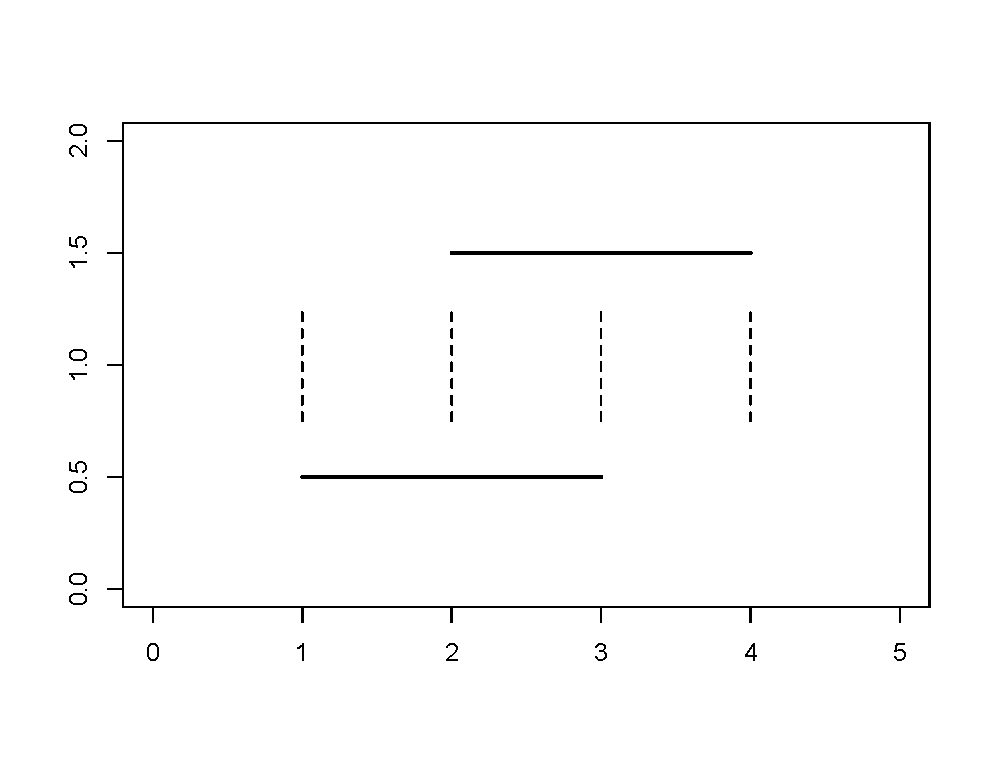
\includegraphics[width = 8cm]{ContrbInt.pdf} }
\caption{Observation intervals and contribution intervals}
\end{figure}	

	\begin{proof}

	Define the $i^{th}$ observation interval $[L_i, R_i]$ to be the interval in which the $i^{th}$ time was known to have occurred. Define a contribution interval to be an interval such that both ends of the interval are ends of an observation interval, with no other ends of observation intervals in between. For example, Figure 2 shows two observation intervals, $L_1 = 1$, $R_1 = 3$ and $L_2 = 2$, $R_2 = 4$. This leads to 3 contribution intervals; [1,2], [2,3] and [3,4]. Note that exchanging mass \emph{between} contribution intervals will affect the likelihood function, but exchanging mass \emph{within} will not. Also, in any area that is not in a contribution interval, $\phi(x)$ needs to be minimized in the LC NPMLE. Thus, $\hat \phi(x)$ will be linear in areas that are between contribution intervals but are not contribution intervals and $\hat \phi(x)$ will be $-\infty$ in areas that are not contribution intervals and not between contribution intervals. 

	For the $i^{th}$ contribution interval, define $l_i$ and $r_i$ to be the end points. For given $\phi(l_i)$, $\phi'(l_i -)$ (left derivative at $l_i$), $\phi(r_i)$ and $\phi'(r_i+)$ (right derivative at $r_i$), this contribution interval affects the likelihood only through the total mass assigned to it, $i.e.$ $p_i = \int_{l_i}^{r_i} e^ {\phi(x)} dx$ (note: under this parameterization, it is not necessary that $\sum p_i = 1$). Note that $p_i$ is minimized by making $\phi(x)$ linear on $(l_i, r_i)$. If $\phi'(l_i - )$ = $\phi'(r_i + )$, then by concavity $\hat{\phi}(x)$ must be linear over $(l_i, r_i)$ and no support points are needed in the interval. If not, we will need to add another support point. Let us define a point inside the contribution interval 	
	\[ m_k = \frac{\phi(r_i) - \phi'(r_i + ) r_i - \phi(l_i) + \phi'(l_i - ) l_i} { \phi'(l_i - ) - \phi'(r_i + )}.
	\]		
	In other words, $m_i$ is the intersection of the linear expansions of $\phi(x)$ from $l_i$ and $r_i$. We can maximize $p_i$ by setting $\phi(m_i)$ to the value of this intersection, as seen in Figure 3. 

	\begin{figure}[h]
\centerline{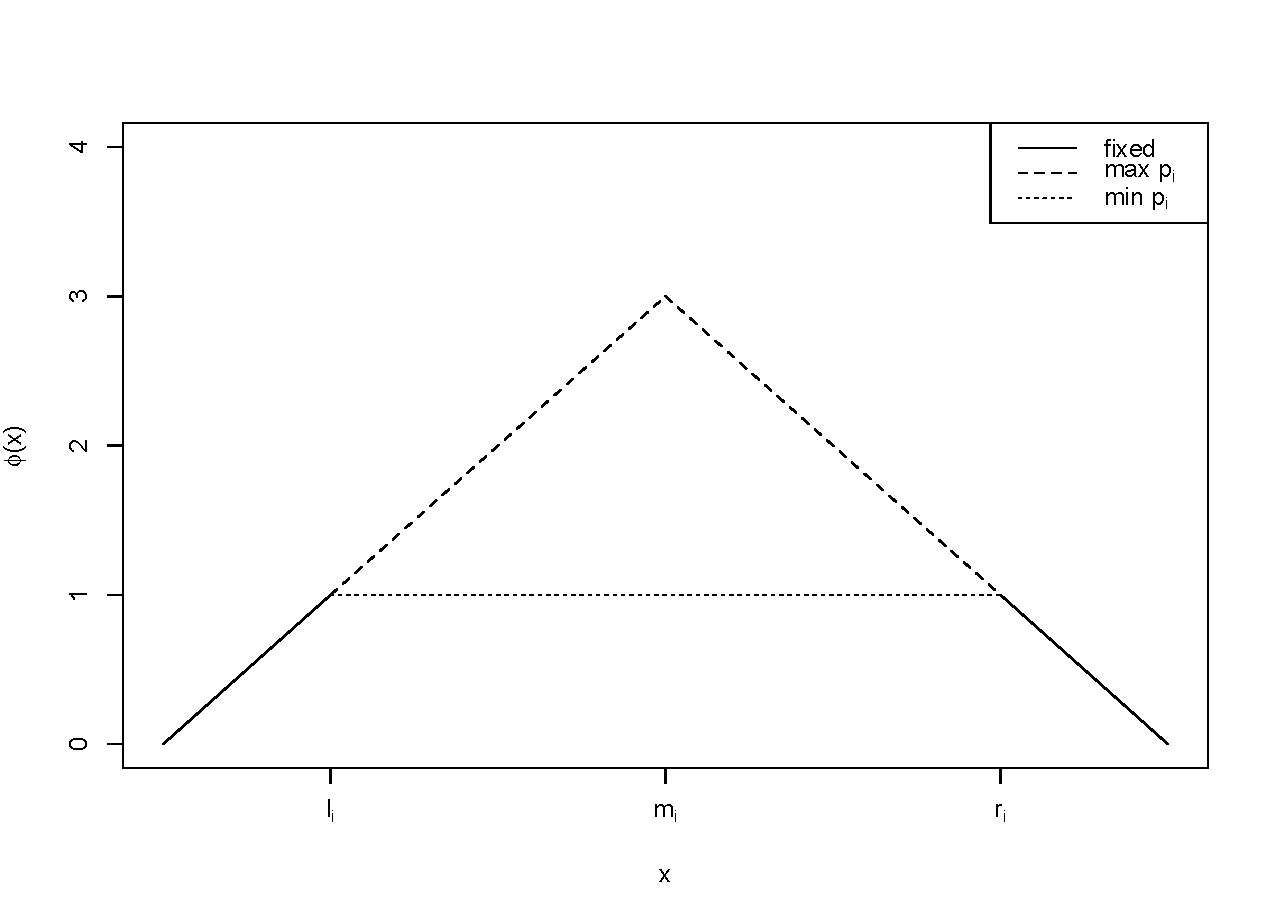
\includegraphics[width = 9cm]{maxminpk.pdf}}
\caption{Maximizing and Minimizing $p_i$}
\end{figure}		

	Therefore, by adding a knot at $m_i$, we can set $p_i$ to either the minimum or the maximum possible under the log concavity constraint, with given $\phi(l_i)$, $\phi'(l_i -)$, $\phi(r_i)$ and $\phi'(r_i+)$. In fact, we can set $p_i$ to any value between the minimum and maximum by setting $\phi(m_i)$ to a suitable value between its minimum and maximum allowed by the constraints.  In other words, whatever likelihood value that can be achieved by an arbitrary log-concave density, we can also achieve it by a piecewise linear function with knots at the end points of contribution intervals and (if needed) one knot inside each contribution interval. This leads to a maximum of $2u-1$ knots.
	\end{proof}
	
	Theorem~\ref{thm1} is important as it clarifies the form of the NPMLE.  However, without knowing $\hat\phi(x)$, one cannot know the exact location of $m_i$ for the $i^{th}$ contribution interval. In order to deal with this, $m_i$ is replaced with the fixed location $mid_i = \frac{l_i + r_i}{2}$ for the main portion of the algorithm, as $mid_i$ should be close to $m_i$. Once the solution is sufficiently close, Newton's method will be used to adjust the location of the knots. 
		
	For the rest of the paper, the {\it support set} refers to all end points and mid points of all the contribution intervals.

	{\section{Parameterizations} }
	
	The algorithm presented in this paper will use an active set algorithm, very similar to the algorithm used in the case of exact times (Rufibach, 2007). In order to clearly define the active set algorithm, several definitions are required. To start with, we define $\beta_i = \phi(x_i)$, where $x_i$ is the $i^{th}$ ordered support point as described in the theorem above. Let $k$ be the number of support points. Because $\phi(x)$ is a linear spline with knots at $x_i$, the values of $\beta_1, \beta_2, ..., \beta_k$ will completely characterize $\phi(x)$. This will be referred to as the simple parameterization. Occasionally, we will refer to the location of $\beta_i$. This refers to $x_i$. We will also denote $\Delta_i = \frac{\beta_{i+1} - \beta_i} {x_{i+1} - x_i}$. With this notation, we will note that the constraint of log concavity is equivalent to $\Delta_1 \geq \Delta_2 \geq ... \geq \Delta_{k-1}$. In principal, we would like to define $x_i$ to be active if $\Delta_{i-1} > \Delta_i$ and inactive if $\Delta_{i-1} = \Delta_i$. However, due to numerical errors in calculating $\Delta_i$, we define $x_i$ to be active if $\Delta_{i-1} > \Delta_i + \xi$ and inactive if $\Delta_{i-1} \leq \Delta_i + \xi$.  We set $\xi = 10^{-13}$ and found no problems resulting from this. 
	
	Similar to the case of exact times (Rufibach 2007), we noticed that the solution tends to have very few active points compared to total number of points considered. We can take advantage of this to create an efficient algorithm using an active set parameterization. Under this parameterization, we treat $\phi(x)$ as a linear spline with knots only at the active points, instead of all the points. We will use the notation $\beta_i^*$ to denote the active set parameterization. The values of the parameters remain the same, i.e. $\beta_i^* = \beta_i$, but when we increase $\beta_i^*$, we also increase the neighboring inactive $\beta_j$ as though the only knots were at the active points, i.e. the inactive $\beta_j$ are determined by linear interpolation from the nearest active points. To illustrate this, figure 4 demonstrates adding 1 to $\beta_4^*$, which takes in inactive point and makes it active under the active set parameterization. To formally characterize addition under the active set parameterization, define $a(i)$ to be the index of the $i^{th}$ active point. If $i = a(m)$ then $\beta_i^{*(t+1)} = \beta_i^{*(t)} + h$ is equivalent to 
		
	\[
	\beta^{(t+1)}_j = 
	\begin{cases}
		\beta^{(t)}_j + h \times \frac{x_j - x_{a(m-1)} } {x_{i} - x_{a(m-1)} } , & \text{if } x_{a(m-1)} < x_j  \leq x_{i} \\ 
		\beta^{(t)}_j + h \times \frac{x_{a(m+1)} - x_j} {x_{a(m+1)} - x_{i} }, & \text{if } x_{ i} < x_j < x_{a(m+1)} \\ 
		\beta^{(t)}_j, & \text{otherwise}
	\end{cases}
	\]

	
\begin{figure}[h]
\centerline{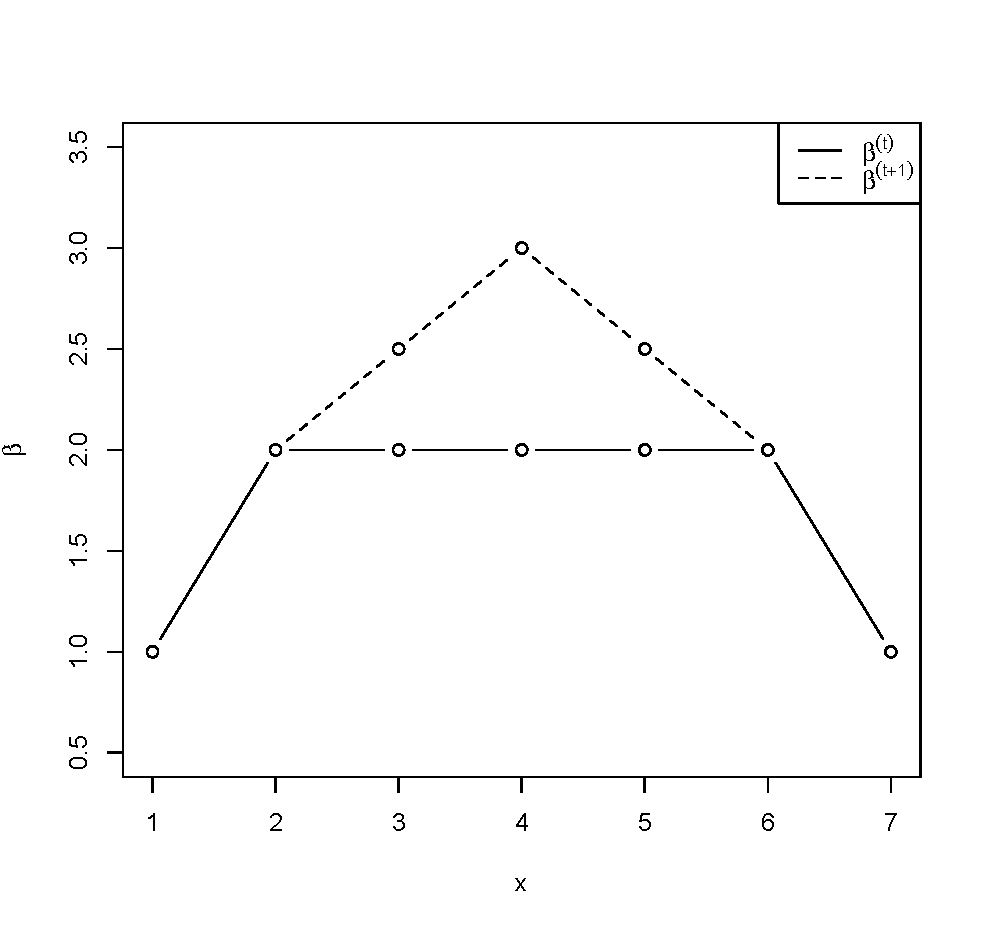
\includegraphics[width = 8cm]{ActivePoint.pdf}}
\caption{$\beta_4^{*(t+1)} = \beta_4^{*(t) }+1$}
\end{figure}		
		
	Under the active set parameterization, all active points have a neighborhood for which they can both increase and decrease without violating the condition of logconcavity. Inactive points have a neighborhood in which they can increase and become an active point, but cannot decrease. In the simple parameterization, inactive points cannot decrease in and all points can increase only if the neighboring points are active. For example, in figure 4, $\beta_4^{(t + 1)} = \beta_4^{(t)} + 1$ violates log concavity, but $\beta_4^{*(t+1)} = \beta_4^{*(t)} + 1$ does not. 
	
	In a slight abuse of notation, let us also define $\Delta_{a(i)} = \frac{\beta_{a(i + 1)} - \beta_{a(i)} } {x_{a(i + 1)} - x_{a(i)} }$. If $K$ = number of active points, then $\Delta_1 \geq \Delta_2 \geq ... \geq \Delta_{k-1}$ is equivalent to $\Delta_{a(1)} \geq \Delta_{a(2)} \geq ... \geq \Delta_{a(K-1)}$. 

			
	{\section{Stopping Criterion} } 
	We discuss the stopping criterion first before presenting the actual iterative algorithm because this discussion clarifies how we characterize the NPMLE, given that it is piecewise log-linear.  Because of the log-concavity constraints, it is natural to consider the KKT conditions (Kuhn and Tucker 1951) which are necessary for an estimate to be a local maximum. Let us define
	
	\[
	\text{KKT error} = {\text{max}} 
	\begin{cases}
		|\frac{\partial \ell } {\partial \beta_i^*}|, & \text{if } \Delta_{i-1} > \Delta_{i} + \xi \\
		\text{max}(\frac{\partial \ell}{\partial \beta_i^*},0 ) , & \text{if } \Delta_{i-1} \leq \Delta_i + \xi \\  
	\end{cases}
	\]
	
	In other words, the error is the maximum of the absolute value of the derivatives associated with the active set parameterization of all the active points and the positive derivatives associated with the active set parameterization of the inactive points (because decreasing would violate the log concavity restraint). 
	
	After the KKT error requirements is met for fixed location of the knots, we allow the knots to move. When this happens, we will have two sources of error: KKT error and error associated with the location of the knots at the active points. Because active points always contain a neighborhood for which the knot can move in either direction, the location error will be the maximum absolute value of the derivative of the log likelihood function as a function of location of each of the active points. This will be referred to as ``location error". At this point in the algorithm, $err$ = max(KKT error, location error). 
	
	The algorithm terminates when either error $<$ tolerance or iteration $>$ max iterations. For this paper, tolerance was set to $10^{-4}$. The reason this value was selected was setting the tolerance to $10^{-5}$ usually required step sizes in the order of $10^{-6}$, which was smaller than the precision of the quadratic programming package we used (see section 6.3 for more discussion). If greater precision was desired, the algorithm still achieves this as the univariate step of the algorithm functions properly even for extremely small step sizes. However, this is much more computationally inefficient and it was decided that the increase in precision was not worth the computational cost. In order to check that using tolerance $10^{-4}$ resulted in solutions sufficiently close to the mode, we simulated 200 data sets of size $n = 200$. In each data set, we set tolerance first to $10^{-4}$ and then $10^{-5}$ and compared final likelihoods of our solutions. In these data sets, it was found that the median increase from using tolerance $10^{-5}$ was $1.6 \times 10^{-9}$ and the maximum increase was found to be 0.0020. 
	
	It is important to note that because the likelihood function is not always concave, this is only a necessary condition for the global maximum, not a sufficient. However, when the algorithm was started from random starting points, it would always converge to the same solutions, suggesting that the issue of non concavity is not too severe. 
	
{\section{Active Set Algorithm} }
	
	{\subsection{Algorithm Outline} } 
	
	
	The algorithm includes four steps: one which selects new points to add to the set of active points (similar to the VDM algorithm of Fedorov 1972), one which efficiently increases the likelihood over the set of currently active points (similar to the methods used to compute the log concave NPMLE with exact observations found in D\"umbgen et al 2011), one that fixes the tails and one that moves the location of the active points. The first step is selects the index $i$ with the maximal error and uses simple univariate techniques to find an optimal $\beta_i^*$. In the second step, maximizing over the active set proceeds by approximating the log-likelihood function with a second order Taylor expansion, and then maximizing this approximation using quadratic programming, similar to the ICM algorithm (Jongbloed 1998).  Because often $\beta_i = -\infty$ on the tails at the solution, it is occasionally necessary to adjust the tails of $\beta$ for numerical stability so this is done in the fixing tails step. Finally, after the solution is sufficient close, we allow the location of the active points to move via Newton's method. The basic form of the algorithm is as follows.
	
	\vspace{3mm}
	
	\begin{itemize}
	
		\item Set $\beta$ (typically $\beta_1 = \beta_2 =...=\beta_k = 0$)
		
		\item Set MOVEX = FALSE
		
		\item While ($err > \epsilon$ and t $<$ max iterations)
		
			\begin{itemize}
			
			\item $t = t + 1$
			
			\item Select index $i$ with maximal KKT error
			
			\item Use univariate optimization to update $\beta_i^*$
						
			\item Use quadratic programming to optimize over active set
			
			\item Fix tails of $\beta$ if necessary
			
			\item Calculate $err$ = KKT error
			
			\item If($err < \epsilon$)
				
				\begin{itemize}
				
				\item MOVEX = TRUE
				
				\end{itemize}
			
			\item If(MOVEX == TRUE)
				
				\begin{itemize}
										
				\item Use bivariate Newton's method to update knot location of active points
				
				\item Calculate $err$ = max(KKT error, location error)
				
				\end{itemize}
			
			\end{itemize}
	
	\item Convert $\beta$ to $e^{\phi(x)} / \int e ^ {\phi(x)} dx$
	
	\item Return $e^{\phi(x)} / \int e ^ {\phi(x)}dx$
	
	\end{itemize}
	
	{\subsection{Univariate Optimization}} 
	
	Our algorithm selects the index $i$ associated with the maximum KKT error. Once the index $i$ is selected, $\beta_i^*$ must be selected which maximizes the likelihood. Let $i = a(j)$ (if $i$ is not an active point, it will be after optimization). From the constraints $\Delta_{a(j-2)} \geq \Delta_{a(j-1)}$, $\Delta_{a(j-1)} \geq \Delta_{a(j)}$ and $\Delta_{a(j)} \geq \Delta_{a(j+1)}$, we derive the constraints
	
	\[ \beta_i^* \leq \text{min}\left(\beta_{a(j-1)} + \Delta_{a(j-2)} \times (x_{a(j)} - x_{a(j-1)}), \beta_{a(j+1)} -\Delta_{a(j+1)} \times (x_{a(j+1)} - x_{a(j)}) \right) 
	\]
	
	\[ \beta_i^* \geq \left(\frac{1}{x_{a(j+1)} - x_{a(j)}} +  \frac{1}{x_{a(j)} - x_{a(j-1)} } \right)^{-1} \times \left(\frac{\beta_{a(j+1)} } { x_{a(j+1)} - x_{a(j)}} + \frac{\beta_{a(j-1)}} {x_{a(j)} - x_{a(j-1)} } \right)
	\]
	
	Constraints which involve an undefined index, such as $a(0)$, can be ignored. If $\frac{d^2 \ell} {d \beta^*_{i} } < 0$, then Newton's method was used, subject to the constraints. Half stepping was used to insure monotonic convergence. Rarely it was observed that $\frac{d^2 \ell} {d \beta^*_{i} } \geq 0$, in which case bisection method was used to update $\beta^*_i$. Although $\ell(\beta^*_i)$ was observed to be non concave, it was not observed to be multimodal.
	
	Much like the VDM algorithm, these steps alone insure that the algorithm will reach a local maximum, but is observed to do so very slowly. Using simulated data with $n = 200$, we observed that using these steps alone frequently failed to converge after 1000 iterations, implying that an algorithm based only on univariate optimization would be insufficient. 
	
	{\subsection{Maximizing Over an Active Set} }
	
	Once given an active set of points, we need a step which can  maximize over the given active set efficiently. Because of the linear constraints of concavity, Newton's method is difficult to apply as it would not respect the boundaries. Instead, an ICM (Jongbloed 1998) algorithm will be used to maximize the over the active set, similar to the algorithm used in the exact case (D\"umbgen et al, 2011). An ICM algorithm works by approximating the target function with a second order Taylor expansion, in which the off diagonal partial derivatives are ignored. Here the parameters considered will be the log density at the active points. It is worth noting that in the traditional ICM algorithm, the off diagonals are ignored due to the expense of computation. In this case the number of parameters considered in our case is actually fairly low, making the number of off diagonals more manageable, but we have other reasons to ignore the off diagonals which will be discussed shortly. This approximation is maximized, according to the linear constraints, via quadratic programming. We will use the notation that a quadratic program minimizes
	
	\[ \frac{1}{2} d^T Q d + c^T d
	\]
	
	Under the constraint \[ A d \leq b\]
	
	Because quadratic programming minimizes a program, we will minimize the Taylor approximation of $-\ell(\beta^*))$, with the off diagonals of the Hessian ignored. In order to have $\frac{1}{2} d^T Q d + c^T d$ be the given approximation, we define
	
	\[ d_i = \beta^{*(t+1)}_{a(i)} - \beta^{*(t)}_{a(i)}
	\]
	
	\[Q_{i,i} = - \frac{\partial^2 \ell(\beta^{*(t)} )} {\partial {\beta^{*(t)}_{a(i)}}^2}
	\]
	 
	\[c_i = -\frac{\partial \ell(\beta^{*(t)})} {\partial \beta_{a(i)}^{*(t)} }
	\]
	
	In order to preserve the constraint of $\Delta_{a(i)} \geq \Delta_{a(i+1)}$, we set 
	
	\[ A_{i,i} = \frac{1}{x_{a(i+1)} - x_{a(i)} }
	\]
	
	\[ A_{i, i + 1} = \frac{-1}{x_{a(i+1)} - x_{a(i)} } + \frac{-1}{x_{a(i+2)} - x_{a(i + 1)} }
	\]
	
	\[ A_{i, i + 2} = \frac{1}{x_{a(i+2)} - x_{a(i + 1)} }
	\]
	
	\[ b_i =\Delta_{a(i + 1)}^{(t)} - \Delta_{a(i)}^{(t)}
	\]
	
	Similar to the ICM algorithm (Jongbloed 1998), half steps will be taken to insure the likelihood function does not decrease. In other words, if $\ell ( \beta^{*(t)} + d ) < \ell ( \beta^{*(t)}  ) $, then $d$ will be replace with $d/2$ until $\ell ( \beta^{*(t)} + d ) \geq \ell ( \beta^{*(t)} )$. It was observed that these half steps were required very infrequently. However, if the tolerance was set very low, such as $10^{-6}$, often this step would fail to increase the likelihood function, as the tolerance for the quadratic solver appeared larger than the necessary step size (the ``solve.QP" function from the R package ``quadprog" was used. Failure typically happened when the largest component of $d$ (before half stepping) was on the order of $10^{-6}$. In such cases, the univariate steps would still work and the algorithm was still observed to converge fairly quickly). 
	
	Perhaps the most novel part of this algorithm is in how we deal with the fact that $\ell(\beta^*)$ may not be locally concave. In order for the standard ICM to work, the function must be locally concave, otherwise the quadratic approximation cannot be maximized. However, occasionally the likelihood function was found to be non-concave. In order to remedy this, an approximation to the second derivative was used which would be concave. Because the ICM algorithm ignores the off diagonals of the Hessian matrix, the only case of concern is when the diagonals of the Hessian are not negative. This was observed to happen occasionally, but less frequently near the solution. Given that the function is bounded from above, a useful approximation of the second derivative can be found which will be guaranteed to be non positive. 
	
	Suppose that the likelihood function is not locally concave as a function of one of the active points, i.e. $ \frac{\partial^2 \ell} { \partial {(\beta^{*(t)}_{a(i)})}^2} \geq 0$. Let $\tilde \beta^*_{a(i)}$ be the value of $\beta^*_{a(i)}$ that maximizes $\ell(\beta^*_{a(i)})$ in the direction of $ \frac{\partial \ell} {\partial \beta^{*(t)}_{a(i)}} $ (i.e. if $  \frac{\partial \ell} {\partial \beta^{*(t)}_{a(i)}} > 0$ only consider  $\tilde \beta^*_{a(i)} > \beta^{*(t)}_{a(i)}$, and if $  \frac{\partial \ell} {\partial \beta^{*(t)}_{a(i)}}< 0 $ only consider $\tilde \beta^*_{a(i)} < \beta^{*(t)}_{a(i)}$)  with all other $\beta_{a(j)}$ held fixed. It is worth noting that we don't require $\tilde \beta^*_{a(i)}$ to respect the boundary set by the constraint of log concavity. If we then consider approximating $\ell(\beta^*_{a(i)})$ with a quadratic function whose first derivative at $\beta^*_{a(i)}$ is $  \frac{\partial \ell} {\partial \beta^{*(t)}_{a(i)}} $ and whose maximum is reached at $\tilde \beta^*_{a(i)}$, this would imply that our approximation of the second derivative would be $\frac{- \left( \frac{\partial \ell} {\partial \beta^{*(t)}_{a(i)} }  \right) } {\tilde \beta^*_{a(i)} -\beta^{*(t)}_{a(i)}}$. This is guaranteed not to be positive.
	
	In the case of a concave likelihood function, half stepping insures that the likelihood function will increase. Because our target function is not locally concave when using this approximation, even half stepping does not insure the likelihood function will increase. If after sufficient half steps (we chose 5), the likelihood still does not increase, this step of the algorithm is skipped. Theoretically, if the ICM step repeatedly failed, the algorithm could be extremely slow due to relying only on the univariate optimization. However, this was not observed to occur and substituting this approximation into the ICM algorithm appears to work very well, usually reducing the number of iterations required to below 100 for simulated data of size $n = 200$. While finding  $\tilde \beta^*_{a(i)}$ does come with some computational cost, this approximation was required infrequently enough and could be done efficiently enough that the computational costs were not significant in the speed of the algorithm. 
	
		{\subsection{Moving the Knots} } 
	
	Recall that we used $mid_k$ as the location of the knots in the center of each contribution interval because we don't know the exact location defined as $m_k$ in our theorem. To optimize the position of the knots, a bivariate Newton's method was used. Two parameters considered were the location of the knot (i.e. $x_i$) and the log density at the knot (i.e. $\beta_i$). While the log likelihood function does appear consistently to be concave as a function of the location of the knots, we already know that the log likelihood is not always concave as a function of $\beta_i$. In the case that the Hessian matrix is not negative definite, we will preform Newton's method on only the location of the knot, as empirically this was always found to be locally concave. The algorithm includes a bisection step, should the likelihood function be non concave as a function of the knot location, but we have not observed it to be necessary. 
	
	It was found that the most computationally efficient way to implement this moving of the knots was to first let the algorithm run without moving the knots until the KKT error was below the tolerance. Once this occurred, then we would add the bivariate Newton's method into the algorithm until both the KKT error and location error were below the tolerance. Once this was satisfied, the algorithm was considered converged. 
	
		{\subsection{Fixing the Tails} }
	
	When computing the log concave NPMLE with exact observations, the area which must have positive mass is known in advance (i.e. the range of all observed times). When computing the log concave NPMLE for interval censored data, this not the case. There will be several contribution intervals which receive 0 mass at the log concave NPMLE. A trivial example is to consider if the data consisted of two overlapping intervals. The log concave NPMLE would place all the mass in the overlap and no mass to the other two surrounding contribution intervals. In the case of the unconstrained NPMLE, the mass was known to be positive only in the set of Turnbull intervals. However, the log concave constraint implies that this is not the case and often some of the contribution intervals outside of the minimum and maximum Turnbull intervals will receive positive mass at the log concave NPMLE, while others will not.
	 		
	Because of this, simply allowing the earlier steps to find the log densities	 at the tails of the estimated density can lead to numerical instability as $\phi(x) \rightarrow -\infty$. Numerical instability typically happened in the range of $\phi(x) = -1000$ for some $x$, as derivatives and second derivatives approached 0. Along with numerical issues is computational cost issues. Consider that if $\phi(x) = -10$ for some $x$, then the density is $4.5 \times 10^{-5}$ times the density at the mode, indicating $\phi(x)$ is very likely $-\infty$ at $\hat \phi(x)$. Even if numerical issues were not observed, allowing the algorithm to meet the stopping criterion can be very computationally expensive for a rather trivial transformation of $\phi(x)$. 
	
	To cope with this, our algorithm would periodically check if setting $\phi(x)$ to $-\infty$ increases the likelihood for $x$ on the tails if $\phi(x) < -t$ for some threshold $t$. If this increased the likelihood, the $\beta_i$ associated would be set to $-\infty$ and either $\beta_{i+1}$ or $\beta_{i-1}$ (depending on which tail) would be check. If setting $\beta_i = -\infty$ did not increase the likelihood, the values would remain unchanged and this part of the algorithm would terminate. Interestingly, choosing $t$ too small leads to local maxes which can be considerably less than the global max, even if optimization techniques are used to check if adding mass back to the tails which have been set to $-\infty$. For poorly chosen $t$, such as $t = 1$, the difference in log likelihood was observed to be as high as 1.5 and the mass could be significantly different on the tails, despite the convergence criterion being satisfied. On the other hand, setting very large $t$, such as 500, was found to increase the number of iterations required several fold. Fortunately, there appears to be a large region for choices of $t$ such that neither issues occurred. The performance across $t$ = 1, 5, 10, 20 and 40 was examined. While it was found that $t = 10$ appeared satisfactory, for robustness $t = 20$ was selected as it lead to a small increase in average iterations (about 15\% more). With this fix, it was found that even with random starting values, the algorithm lead to the same estimate. 
		
	{\section{Motivating Example} }
	
	For a motivating example, we will borrow data from MacMahon and Worcestor (1966). Questionnaires were collected from $n = 2423$ participants regarding age at menopause. Because several of the subjects had not experienced menopause yet, this data set contained right censored data. However, MacMahon and Worcestor (1966) found that there was a marked terminal digit clustering in the response of reported time of menopause. Because of this, Krailo and Pike (1983) recommended only using the menopausal status of women at the time of the questionnaire, thus resulting in current status data. The data also contains two types of menopause; operative menopause and natural menopause. 
	
	Earlier analyses of this data used a competing risks model (Jewell et al 2003). For demonstrative purposes, we will only examine the time to menopause, irregardless of the type of menopause. For this example, we will examine the estimated densities and survival curves, although clearly it would be simple to also examine the estimated hazard as well. We wanted to compare the log concave estimate to the unconstrained NPMLE, the logspline estimator and the kernel density estimator. However, using the standard settings found in the CRAN logspline package, the logspline estimator failed to converge with this dataset, a common problem for the log spline estimator with current status data. When using the kernel smoother, the problem of selecting bandwidth was non trivial. Braun et al (2005) suggest using cross validation for selecting bandwidth. However, with a dataset of this size, this is not an option. Instead, midpoint imputation was used to determine bandwidth, as demonstrated in the CRAN ICE package. Other ad hoc fixes are left endpoint and right endpoint imputation. All of these lead to relatively close bandwidths, which lead to very similar estimates. 
		
\begin{figure}[h]
\centerline{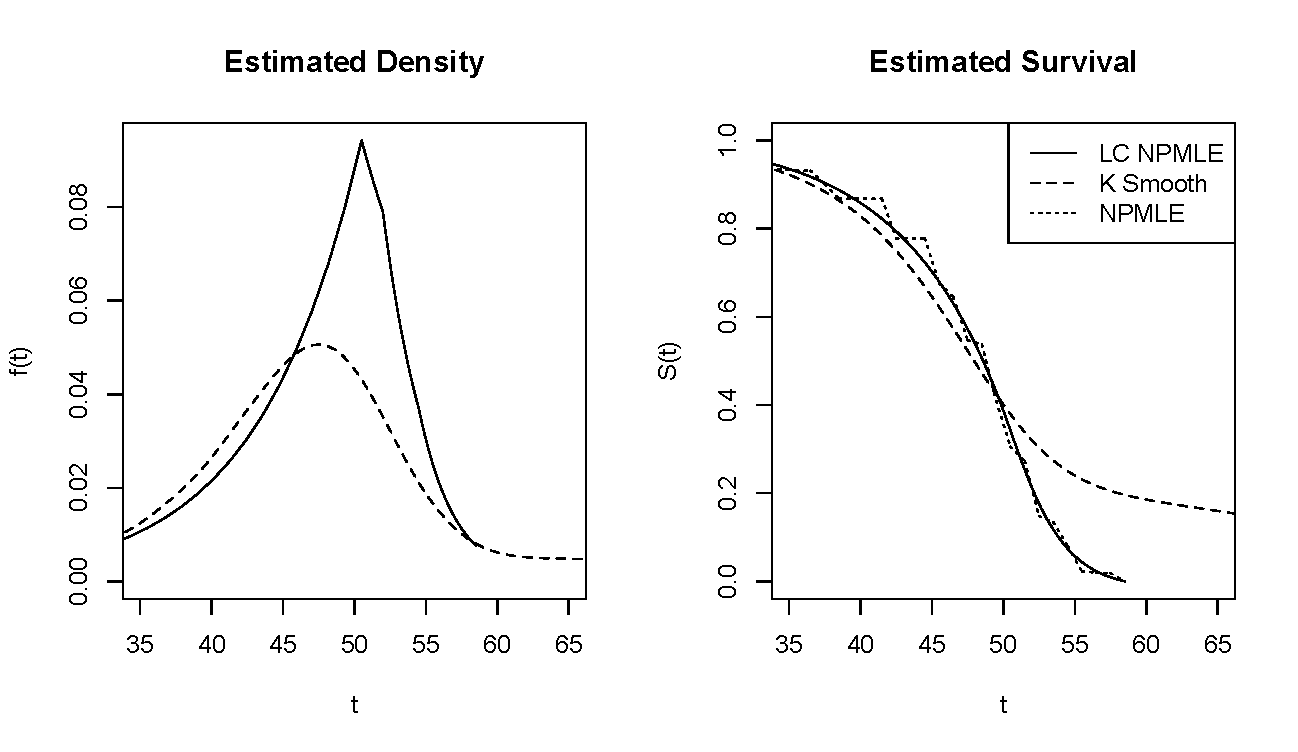
\includegraphics[width = 12cm]{MenoPlot.pdf}}
\caption{Estimated Functions}
\end{figure}		
	
	Plotted estimates can be seen in figure 5 for the menopause data. The full estimator is not shown, in order to be able to see the estimator in better detail. The full estimator can been in figure 6 in the appendix. A few key features we see is that the log concave NPMLE has a much more jagged density estimator than the kernel smoother. This can be seen as a disadvantage for the log concave NPMLE where smoothness of the estimated density is a priority. We also note that while the log concave NPMLE and the unconstrained NPMLE survival estimates appear consistent with each other, there is a large disagreement with those estimates and the kernel smoother's. The log concave NPMLE places 0 masses beyond t = 58.5, while the kernel smoother places mass as far as t = 100. The NPMLEs appear to agree with what is known about menopause, while the kernel smoother appears to be a less accurate portrayal of the distribution of time to menopause. For example, Treloar 1981 presents data from a longitudinal study. Excluding the cases lost to follow up, all 729 cases had experienced menopause by age 59 (and only one had experienced menopause after 58). However, the kernel smoother estimates that $S(59) =  0.19$. In contrast, both the log concave NPMLE and unconstrained NPMLE place 0 mass beyond 58.5, which agree much better with Treloar's findings. The current implementation of the LC NPMLE algorithm took 0.57 seconds to converge, although it is very important to note that this the best case scenario for a data set of this size (see appendix on acceleration from ties). In contrast, the kernel smoother took 16.5 seconds and the unconstrained NPMLE algorithm, as implemented in the CRAN package  MLEcens, took 0.139 seconds to converge. 
	
	
	{\section{Simulations} } 
	
	Now that a reasonably fast algorithm has been created for computing the log concave NPMLE, the finite sample size operating characteristics can be examined and compared to the competing estimators. In order to examine which estimator performed best in estimating quantiles, the bias and standard deviation of the estimated 0.1, 0.25, 0.5, 0.75 and 0.9 quantiles were compared across the estimators. 
			
	Current status data was used, as this simplified the process of censoring. The true time $T$ was simulated along with the censoring time $C$. For simplicity, $C$ followed the same distribution as $T$. The only information kept was $C$ and whether the event was right or left censored. If $T_i$ was right censored, $R_i$ was set to the maximum value of $C \times 1.1$.

	A variety of different distributions were used to examine how the estimators worked in different scenarios. The distributions tested were gamma(shape = 2, rate = 2), gamma(shape = 100, rate = 2), weibull(shape = 6, scale = 4),  lognormal($\mu = 0$, $\sigma = 1$) and a gamma mixture with p = (0.5, 0.5), component 1 = gamma(shape = 2, rate = 2), component 2 = gamma(shape = 5, rate = 1). It should be noted that the last two simulations violate the assumption of log concavity; the log normal distribution is mildly non log concave due to heavy tails, while the gamma mixture model is heavily non log concave due to bimodality. In each of the simulations, datasets were generated with $n$ = 50, 200 and 800. For $n$ = 50 and 200, MC = 400 simulations were generated. For $n$ = 800, MC = 100 simulations were generated.
	
	Tables of the results are given in the appendix. We refer to the log concave NPMLE as the LC NPMLE and the unconstrained NPMLE as the UC NPMLE. Some general trends that were noted from the simulations were:
	
\vspace{3mm}	
	
\begin{itemize}	
		
	\item For log concave data, the LC NPMLE always outperforms the UC NPMLE in both bias and standard deviation.
	
	\item For log concave data, the LC NPMLE consistently outperforms the kernel smoother in terms of bias in quantile estimation. Quite often, the bias from the kernel smoother was non-trivial. 
				
	\item The kernel smoother shows extreme bias when the censored intervals cover vast regions where the density is very close to 0, such as the gamma (100,2) case. Again, this bias from the kernel smoother appears to increase as $n$ increases. This bias is thought to be the cause of the discrepancy in estimates for the motivating example. 
	
	\item For log concave data, the bias approaches 0 fairly quickly for the LC NPMLE. For samples over 200, the largest bias to standard deviation ratio was 0.4, although for $n$ = 50, we observe a bias to standard deviation ratio of 0.7. 
	
	\item For log concave data, the LC NPMLE has higher standard deviation than the kernel smoother in small data sets. This trend reversed in larger datasets

	\item For log normal data, significant bias was observed in the estimation of the upper tail for the LC NPMLE. While this bias reduced as $n$ increased, it did not appear to be converging to 0. While the UC NPMLE showed significant bias in small samples, the bias appeared to be converging to 0. The kernel smoother observed heavier bias than the LC NPMLE in estimating all cases except estimating the 0.9 quartile with $n$ = 50. 
		
	\item For mixture gamma data, significant bias was observed for almost all quantiles for the LC NPMLE, although this was about equal for the kernel smoother. While the UC NPMLE suffered from significant bias in $n$ = 50, by $n = 200$, these biases were mostly insignificant.
		
	\item For density estimation, the trend was very consistent; the log concave NPMLE displayed lower bias but significantly higher standard deviation than the kernel smoother. The bias from the kernel smoother was often substantial. This bias often did not decrease with an increase in sample size. 
	
	\item While the log concave NPMLE did well in terms of bias, the standard deviation was often so high that it would be unreasonable to use for density estimation unless the data set was quite large ($n \geq 800$). 
\end{itemize}	

	These simulation results suggest that the log concave NPMLE would be the estimator of choice for quantile estimation with current status data that was believed to be log concave or even mildly non logconcave. The advantage of the log concave estimator increases as $n$ increases. In large data sets or moderately sized data sets with light case II interval censoring, the log concave NPMLE may be reasonable for density estimation, but it is not recommended for smaller data sets ($n < 800$ for current status data).
	
	{\section{Future Work} } 

	Uniqueness of the solution has not been shown yet. In the case of the log concave NPMLE for exact data, uniqueness is shown using the fact that the log likelihood is strictly convex (Rufibach 2007). In the case of the univariate unconstrained NPMLE, it has been shown that the solution does not have mixture non-uniqueness (for a solution set of intervals, there is only one assignment of mass to each interval which maximizes the likelihood function) but does suffer from representational non-uniqueness (for a mixed mass and interval, any assignment of mass within the interval leads to the same likelihood, Gentleman and Vandal 2001). The proof depends on the fact that the solution only assigns mass to the Turnbull intervals. Neither of these proofs can be easily extended to the log concave NPMLE. 
	
	There are several trivial example of representational non-uniqueness for the log concave NPMLE, although it is very easy to show that it must have much less of an affect on the log concave NPMLE than on the constrained NPMLE. This is because representational non-uniqueness can only occur in contribution intervals with active points, as $\hat \phi(x)$ will be strictly linear in intervals that do not contain an active point. It is not clear whether $\hat \phi(x)$ could have mixture non-uniqueness; the proof of that the unconstrained NPMLE does not suffer from mixture non-uniqueness in the univariate case requires the fact mass will only be assigned to maximal intersections, which is not true for the log concave NPMLE. To investigate whether mixture non-uniqueness could be an issue, the algorithm was run several times from random initial values but always found to converge to the same solution for each simulated data set, suggesting that mixture non-uniqueness may not occur for the log concave NPMLE. However, no theoretic proof of this exists at this time.
	
	Although the algorithm presented in this paper is acceptable for small to moderate sized data sets or larger data sets with large amounts of ties (see appendix), it would be too slow for larger data sets with large numbers of unique values. For example, in our simulations we found that if $n = 5,000$, all with unique times, the algorithm look over 2 minutes to converge on average (see table 1). In contrast, the CRAN package ``MLEcens" can compute the unconstrained NPMLE for $ n = 5,000$ in 3.85 seconds on average. 
	
	In section 6.5, it is noted that the algorithm can find local maximum, returning an estimate which can differ significantly from the true MLE on the tails. While an ad hoc fix is presented, it would be preferable to find a transformation of $\phi(x)$ such that the estimate could step away from the local max and toward the global max. Such a step would likely have to be consider both the length of the tails of $\phi(x)$ and the log density of the tails of $\phi(x)$ simultaneously. Adding such a step would likely both accelerate the algorithm and help insure convergence to the global maximum.  
		
	Now that an algorithm has been developed which can handle moderate sized data sets, several important questions about the operating characteristics of the LC NPMLE must be addressed. Two topics unique to this estimator are that must be addressed is assessing the bias resulting from violation of the logconcave assumption and creating a test of log concavity. We present two potential methods of testing the log concavity assumption. The first would involve computing the integrated squared difference between the unconstrained NPMLE and the logconcave NPMLE survival function. In order to sample from the null distribution, censored samples can be taken from the log concave NPMLE estimated distribution and the unconstrained and log concave NPMLEs can be estimated. A second approach could be a likelihood ratio test, in which the maximum log concave likelihood would be compared to the maximum unconstrained likelihood. Because the solution would be on the boundary, the distribution of the test statistic under the null hypothesis is not trivial. More work is required to assess the validity of these tests.  


{\section{Appendix} } 



	{\subsection{Simulation Results} }

	{\subsubsection{Average Computation Times} } 
	
	To investigate the speed of our algorithm, we computed the LC NPMLE across different scenarios. As stated above, the complexity of the algorithm is not only a function of sample size, but also the number of unique times in the data. Theoretically each step should be $O(u^2)$, where $u$ is the number of unique times. While given $u$, $n$ does not affect the complexity of each iteration, empirically we see that the number of iteration increases with $n$ for a fixed $u$. On Table 1, we present average computation time in seconds across different sample sizes and different numbers of unique times in the data using simulated current status data from a gamma(2,2) distribution. Binning was used to create the number of unique times. 
	
	\begin{table}[H]

\begin{center}	
\caption{Average Computation Times (in seconds)}

\begin{tabular} {| c | c | c | c | c | c | c | c |} 


	 \hline

		 & \multicolumn{7} {|c|} {Unique Times} \\
		
	\hline	
		
	$n$ & 10 & 50 & 100 & 500 & 1000 & 2000 & 5000\\	
		
	 \hline 
 
 	100 & 0.07 & 0.15 & 0.17 & NA & NA &  NA & NA\\ 
	
	\hline
	
	500 & 0.19 & 0.27 & 0.46 & 0.86 & 2.44 & NA & NA\\
	
	\hline
	
	5000 & 0.42 & 0.86 & 1.11 & 5.07 & 7.59 & 31.6 & 156\\ 
	
	\hline
	
\end{tabular}
\end{center}

\end{table}

	
	{\subsubsection{Quantile Estimation} } 
	
		The tables below give the results of the simulation for quantile estimation. The top of the table shows the 0.1, 0.25, 0.5, 0.75 and 0.9 quantile, respectively, of the distribution of the simulated data. The simulated data was current status data, in which the distribution of the censoring distribution followed the same distribution as the true times. The main table shows the bias and standard deviation found for each of the estimators, organized by sample size. LC = log concave NPMLE, UC = unconstrained NPMLE and KS = Kern Smoother.
	


\begin{table}[H]

\begin{center}	
\caption{Quantile Estimation for Gamma(2, 2)}

\begin{tabular} {| c | c | c | c | c | c | c | } 


	 \hline
		&Q(p)&	0.27 (0.1)&	0.48 (0.25)&	0.84 (0.5)&	1.35 (0.75)&	1.94 (0.9)\\ 
 \hline 
 	$n$ & & \multicolumn{5}{|c|}{Bias / Standard Deviation} 
 \\ 
 \hline 
\multirow{3}{*}{50}		&	LC	&-0.04/0.11	&-0.04/0.11	&-0.04/0.14	&0.01/0.22	&0.21/0.31\\ 
			&	UC	&-0.11/0.14	&-0.07/0.17	&-0.05/0.22	&0.02/0.33	&0.27/0.4\\ 
			&	KS	&0.03/0.07	&-0.03/0.09	&-0.07/0.13	&-0.1/0.24	&-0.11/0.37\\ 
	\hline 
\multirow{3}{*}{200}		&	LC	&-0.01/0.07	&-0.01/0.06	&-0.02/0.08	&-0.01/0.13	&0.07/0.21\\ 
			&	UC	&-0.05/0.09	&-0.02/0.12	&-0.03/0.14	&0/0.22	&0.12/0.35\\ 
			&	KS	&0.02/0.04	&-0.01/0.05	&-0.02/0.07	&-0.05/0.14	&-0.28/0.35\\ 
	\hline 
\multirow{3}{*}{800}		&	LC	&0/0.03	&0/0.03	&-0.01/0.04	&-0.01/0.06	&0.03/0.11\\ 
			&	UC	&0/0.05	&-0.02/0.06	&-0.01/0.08	&0.01/0.14	&0.05/0.21\\ 
			&	KS	&0.01/0.02	&0/0.02	&0/0.04	&-0.02/0.07	&-0.47/0.29\\ 
	\hline 

\end{tabular}
\end{center}

\end{table}


\begin{table} [H]

\begin{center}
\caption{Quantile Estimation Gamma(100, 2)}

\begin{tabular} {| c | c | c | c | c | c | c | } 

	 \hline
		&Q(p)&	43.7 (0.1)&	46.5 (0.25)&	49.8 (0.5)&	53.3 (0.75)&	56.5 (0.9)\\ 
 \hline 
 	$n$ & & \multicolumn{5}{|c|}{Bias / Standard Deviation} 
 \\ 
 \hline 
\multirow{3}{*}{50}		&	LC	&-0.4/2.55	&-0.08/1.54	&-0.05/1.14	&0.06/1.44	&0.72/2.14\\ 
			&	UC	&-0.67/3.73	&-0.23/2.08	&-0.21/1.75	&0.03/2.03	&0.93/2.41\\ 
			&	KS	&11.48/7.22	&3.36/3.15	&-0.1/1.51	&-2.24/1.56	&-3.89/1.92\\ 
	\hline 
\multirow{3}{*}{200}		&	LC	&-0.1/1.13	&0.08/0.73	&-0.02/0.67	&-0.1/0.81	&0.18/1.19\\ 
			&	UC	&-0.17/1.51	&0.04/1.1	&-0.11/1.06	&-0.01/1.23	&0.14/1.82\\ 
			&	KS	&12.64/5.73	&1.88/1.33	&-0.22/0.67	&-1.69/0.93	&-3.83/1.6\\ 
	\hline 
\multirow{3}{*}{800}		&	LC	&0.14/0.68	&0.04/0.44	&-0.07/0.33	&-0.12/0.44	&0/0.61\\ 
			&	UC	&0.1/0.97	&-0.03/0.64	&-0.1/0.51	&-0.05/0.75	&-0.04/0.98\\ 
			&	KS	&15.94/3.23	&1.18/0.66	&-0.25/0.3	&-1.22/0.48	&-4.57/1.35\\ 
	\hline 

\end{tabular}
\end{center}

\end{table}

\begin{table}[H]

\begin{center}
\caption{Quantile Estimation for Weibull(6, 4)}

\begin{tabular} {| c | c | c | c | c | c | c | } 

	 \hline
		&Q(p)&	2.75 (0.1)&	3.25 (0.25)&	3.76 (0.5)&	4.22 (0.75)&	4.6 (0.9)\\ 
 \hline 
 	$n$ & & \multicolumn{5}{|c|}{Bias / Standard Deviation} 
 \\ 
 \hline 
\multirow{3}{*}{50}		&	LC	&-0.12/0.33	&-0.02/0.21	&0/0.15	&0.01/0.18	&0.06/0.25\\ 
			&	UC	&-0.24/0.38	&-0.09/0.29	&-0.03/0.23	&0.05/0.24	&0.17/0.26\\ 
			&	KS	&0.5/0.44	&0.19/0.26	&0.01/0.16	&-0.13/0.17	&-0.25/0.19\\ 
	\hline 
\multirow{3}{*}{200}		&	LC	&-0.03/0.18	&0.01/0.12	&0/0.09	&0/0.09	&0.02/0.14\\ 
			&	UC	&-0.1/0.25	&-0.05/0.2	&-0.02/0.16	&0.02/0.15	&0.08/0.19\\ 
			&	KS	&0.51/0.31	&0.12/0.14	&0.01/0.09	&-0.09/0.1	&-0.25/0.14\\ 
	\hline 
\multirow{3}{*}{800}		&	LC	&0/0.11	&0.01/0.06	&0/0.05	&-0.01/0.05	&0/0.07\\ 
			&	UC	&-0.03/0.19	&-0.01/0.12	&-0.02/0.11	&0/0.1	&0.02/0.12\\ 
			&	KS	&0.55/0.17	&0.08/0.06	&0/0.04	&-0.07/0.05	&-0.3/0.1\\ 
	\hline 

\end{tabular}
\end{center}
\end{table}

\begin{table}[H]

\begin{center}
\caption{Quantile Estimation for Lognormal(0, 1)}
  
\begin{tabular} {| c | c | c | c | c | c | c | } 

	 \hline
		&Q(p)&	0.28 (0.1)&	0.51 (0.25)&	1 (0.5)&	1.96 (0.75)&	3.6 (0.9)\\ 
 \hline 
 	$n$ & & \multicolumn{5}{|c|}{Bias / Standard Deviation} 
 \\ 
 \hline 
\multirow{3}{*}{50}		&	LC	&-0.04/0.13	&-0.09/0.15	&-0.14/0.23	&0.02/0.43	&0.77/0.73\\ 
			&	UC	&-0.12/0.17	&-0.11/0.23	&-0.12/0.4	&-0.04/0.94	&0.59/1.95\\ 
			&	KS	&0.18/0.21	&-0.11/0.13	&-0.35/0.29	&-0.49/0.7	&-0.54/1.56\\ 
	\hline 
\multirow{3}{*}{200}		&	LC	&0/0.07	&-0.03/0.07	&-0.08/0.12	&-0.02/0.25	&0.49/0.46\\ 
			&	UC	&-0.05/0.09	&-0.03/0.13	&-0.07/0.24	&-0.01/0.5	&0.27/1.05\\ 
			&	KS	&0.16/0.16	&-0.08/0.07	&-0.26/0.18	&-0.28/0.37	&-0.58/1.09\\ 
	\hline 
\multirow{3}{*}{800}		&	LC	&0/0.03	&-0.02/0.03	&-0.07/0.06	&-0.04/0.12	&0.39/0.22\\ 
			&	UC	&-0.03/0.06	&-0.03/0.07	&0/0.14	&-0.04/0.33	&0.08/0.83\\ 
			&	KS	&0.1/0.06	&-0.08/0.03	&-0.19/0.11	&-0.13/0.18	&-0.78/0.91\\ 
	\hline 

\end{tabular}

\end{center}
\end{table}

\begin{table}[H]

\begin{center}
\caption{Quantile Estimation for Gamma Mixture}

\begin{tabular} {| c | c | c | c | c | c | c | } 

	 \hline
		&Q(p)&	0.41 (0.1)&	0.84 (0.25)&	2.17 (0.5)&	4.68 (0.75)&	6.72 (0.9)\\ 
 \hline 
 	$n$ & & \multicolumn{5}{|c|}{Bias / Standard Deviation} 
 \\ 
 \hline 
\multirow{3}{*}{50}		&	LC	&-0.14/0.22	&-0.36/0.31	&-0.27/0.53	&0.51/0.79	&0.95/1.03\\ 
			&	UC	&-0.26/0.33	&-0.28/0.57	&-0.3/1.02	&0.17/1.31	&0.96/1.43\\ 
			&	KS	&-0.02/0.21	&-0.42/0.28	&-0.43/0.51	&0.09/0.9	&0.01/1.26\\ 
	\hline 
\multirow{3}{*}{200}		&	LC	&-0.03/0.11	&-0.21/0.14	&-0.14/0.27	&0.39/0.43	&0.32/0.63\\ 
			&	UC	&-0.09/0.18	&-0.09/0.3	&-0.2/0.77	&0.07/0.89	&0.43/1.09\\ 
			&	KS	&-0.04/0.09	&-0.28/0.13	&-0.15/0.26	&0.23/0.53	&-0.51/1.01\\ 
	\hline 
\multirow{3}{*}{800}		&	LC	&0.01/0.05	&-0.15/0.07	&-0.08/0.13	&0.38/0.22	&0.04/0.35\\ 
			&	UC	&-0.05/0.11	&-0.05/0.15	&-0.04/0.45	&0.04/0.53	&0.07/0.79\\ 
			&	KS	&-0.05/0.04	&-0.18/0.06	&0.03/0.14	&0.31/0.26	&-0.97/0.64\\ 
	\hline 

\end{tabular}
\end{center}
\end{table}
	
	
	{\subsubsection{Density Estimation} } 
	
	The tables below give the results of the simulation for density estimation at the quantiles. The top of the table shows the density of the simulated data at the  0.1, 0.25, 0.5, 0.75 and 0.9 quantiles. The simulated data was current status data, in which the distribution of the censoring distribution followed the same distribution as the true times.The main table shows the bias and standard deviation found for each of the estimators, organized by sample size. LC = log concave NPMLE and KS = Kern Smoother. The unconstrained NPMLE is excluded as it does not provide density estimates. 

	
	
\begin{table}[H]
\begin{center}	

\caption{Density Estimation at Quantiles for Gamma (2,2) }
	
\begin{tabular} {| c | c | c | c | c | c | c | } 

	 \hline
		&f(p)&	0.62(0.1)&	0.74(0.25)&	0.63(0.5)&	0.36(0.75)&	0.16(0.9)\\ 
 \hline 
 	$n$ & & \multicolumn{5}{|c|}{Bias / Standard Deviation} 
 \\ 
 \hline 
\multirow{3}{*}{50}		&	LC	&0.11/0.35	&-0.01/0.31	&-0.04/0.21	&-0.09/0.22	&0.01/0.13\\ 
			&	KS	&0.15/0.1	&0.12/0.11	&0.01/0.1	&-0.02/0.08	&-0.02/0.07\\ 
	\hline 
\multirow{3}{*}{200}		&	LC	&-0.05/0.27	&0/0.15	&0/0.11	&-0.03/0.08	&-0.02/0.09\\ 
			&	KS	&0.09/0.08	&0.05/0.07	&-0.01/0.08	&0.02/0.05	&0.02/0.03\\ 
	\hline 
\multirow{3}{*}{800}		&	LC	&-0.05/0.12	&0.01/0.09	&0.01/0.07	&-0.01/0.04	&-0.02/0.04\\ 
			&	KS	&0.05/0.04	&0.01/0.04	&-0.01/0.04	&0.05/0.03	&0.05/0.02\\ 
	\hline 

\end{tabular}
\end{center}	
	
\end{table}	
	
	
\begin{table}[H]

\begin{center}	

\caption{Density Estimation at Quantiles for Gamma(100,2)}

\begin{tabular} {| c | c | c | c | c | c | c | } 

	 \hline
		&f(p)&	.038(0.1)&	.067(0.25)&	.08(0.5)&	.061(0.75)&	.032(0.9)\\ 
 \hline 
 	$n$ & & \multicolumn{5}{|c|}{Bias / Standard Deviation} 
 \\ 
 \hline 
\multirow{3}{*}{50}		&	LC	&.007/.029	&-.007/.036	&-.003/.029	&-.006/.034	&.003/.026\\ 
			&	KS	&.01/.005	&.027/.007	&.032/.008	&.016/.007	&-.003/.006\\ 
	\hline 
\multirow{3}{*}{200}		&	LC	&-.004/.022	&-.002/.018	&.003/.016	&-.002/.015	&-.006/.018\\ 
			&	KS	&.012/.003	&.023/.005	&.023/.007	&.012/.005	&0/.004\\ 
	\hline 
\multirow{3}{*}{800}		&	LC	&-.002/.01	&.003/.009	&0/.013	&-.001/.009	&-.004/.009\\ 
			&	KS	&.017/.002	&.022/.003	&.014/.006	&.01/.004	&.005/.002\\ 
	\hline 

\end{tabular}
\end{center}
\end{table}
	
	
\begin{table}[H]

\begin{center}
\caption{Density Estimation at Quantiles for Weibull(6,4)}
\begin{tabular} {| c | c | c | c | c | c | c | } 

	 \hline
		&f(p)&	0.21(0.1)&	0.4(0.25)&	0.55(0.5)&	0.49(0.75)&	0.3(0.9)\\ 
 \hline 
 	$n$ & & \multicolumn{5}{|c|}{Bias / Standard Deviation} 
 \\ 
 \hline 
\multirow{3}{*}{50}		&	LC	&0.02/0.16	&-0.05/0.23	&-0.02/0.19	&-0.04/0.27	&0.02/0.23\\ 
			&	KS	&0.02/0.04	&0.07/0.07	&0.11/0.09	&0.09/0.07	&0/0.06\\ 
	\hline 
\multirow{3}{*}{200}		&	LC	&-0.04/0.11	&-0.01/0.09	&0.01/0.1	&-0.02/0.13	&-0.03/0.17\\ 
			&	KS	&0.04/0.03	&0.06/0.05	&0.08/0.06	&0.08/0.05	&0.03/0.04\\ 
	\hline 
\multirow{3}{*}{800}		&	LC	&-0.01/0.05	&0/0.06	&0.01/0.07	&0/0.08	&-0.03/0.08\\ 
			&	KS	&0.05/0.02	&0.06/0.03	&0.05/0.04	&0.08/0.03	&0.06/0.02\\ 
	\hline 

\end{tabular}
\end{center}
\end{table}	

\begin{table}[H]
\begin{center}

\caption{Density Estimation at Quantiles for Lognormal(0,1)}

\begin{tabular} {| c | c | c | c | c | c | c | } 

	 \hline
		&f(p)&	0.63(0.1)&	0.62(0.25)&	0.4(0.5)&	0.16(0.75)&	0.05(0.9)\\ 
 \hline 
 	$n$ & & \multicolumn{5}{|c|}{Bias / Standard Deviation} 
 \\ 
 \hline 
\multirow{3}{*}{50}		&	LC	&0.17/0.28	&0.06/0.21	&-0.04/0.12	&-0.06/0.09	&0/0.04\\ 
			&	KS	&0.35/0.07	&0.28/0.09	&0.03/0.08	&-0.05/0.04	&-0.01/0.03\\ 
	\hline 
\multirow{3}{*}{200}		&	LC	&0.03/0.16	&0.07/0.09	&0/0.05	&-0.04/0.03	&-0.01/0.02\\ 
			&	KS	&0.32/0.06	&0.25/0.08	&0.01/0.06	&-0.05/0.03	&0/0.02\\ 
	\hline 
\multirow{3}{*}{800}		&	LC	&0.02/0.08	&0.06/0.05	&0.01/0.02	&-0.03/0.01	&-0.01/0.01\\ 
			&	KS	&0.29/0.05	&0.21/0.07	&-0.02/0.04	&-0.04/0.03	&0.01/0.01\\ 
	\hline 

\end{tabular}
\end{center}
\end{table}

\begin{table}[H]
\begin{center}
\caption{Density Estimation at Quantiles for Gamma Mixture}

\begin{tabular} {| c | c | c | c | c | c | c | } 

	 \hline
		&f(p)&	0.36(0.1)&	0.32(0.25)&	0.11(0.5)&	0.09(0.75)&	0.05(0.9)\\ 
 \hline 
 	$n$ & & \multicolumn{5}{|c|}{Bias / Standard Deviation} 
 \\ 
 \hline 
\multirow{3}{*}{50}		&	LC	&0.13/0.11	&0.08/0.08	&-0.07/0.04	&-0.01/0.04	&0.01/0.03\\ 
			&	KS	&0.21/0.03	&0.13/0.04	&-0.07/0.03	&0.01/0.02	&0.01/0.02\\ 
	\hline 
\multirow{3}{*}{200}		&	LC	&0.09/0.05	&0.07/0.03	&-0.06/0.01	&0.01/0.01	&0.01/0.01\\ 
			&	KS	&0.18/0.03	&0.08/0.03	&-0.07/0.02	&0.02/0.02	&0.01/0.01\\ 
	\hline 
\multirow{3}{*}{800}		&	LC	&0.08/0.02	&0.07/0.02	&-0.06/0.01	&0.01/0.01	&0.01/0.01\\ 
			&	KS	&0.13/0.02	&0.04/0.02	&-0.05/0.01	&0.02/0.01	&0.02/0\\ 
	\hline 

\end{tabular}
\end{center}
\end{table}
		
	{\subsection{Efficient Likelihood Functions} } 	
	
	For this algorithm, efficient calculation of the likelihood and derivatives is paramount for an efficient algorithm. The first step in calculating the likelihood function is calculating a vector {\bf p} in which $p_k = \int_{t_k}^{t_{k+1}} e^ { \phi(x) } \,dx$, or the mass placed within the $k^{th}$ contribution interval. Because $\phi(x)$ is linear between the knots, the solution is in closed form. Define $\phi(t_k) = \phi_k$ and $\Delta x_k = x_{k+1} - x_k$. Integrating gives us 
	
	\[ p_k = \frac{\Delta t_k} {\Delta \phi_k } \times (e^{\phi_{k+1} } - e^{\phi_k } ) 
	\]
	
	This is undefined if $\phi_{k+1} = \phi_k$ and so the limit as $\phi_{k+1} \rightarrow \phi_k$ will be used instead. The limit is $e^{\phi_k} \times \Delta t_k$. It was also observed that calculating $p_k$ suffers from numeric instability as $\phi_k \rightarrow \phi_{k+1}$. In order to deal with, if $|\Delta\phi_k | < 10^{-5}$, $p_k$ will be replaced with a first order Taylor approximation, i.e., 
	
	\[ p_k \approx e^{\phi_k} \times \Delta t_k + \frac{\partial p_k}{\partial \phi_{k+1}} \times \Delta \phi_k 
	\]
	\[
	= e^{\phi_k} \times \Delta t_k + e^{\phi_k} \times \frac {\Delta t_k} {2} \times \Delta \phi_k
	\]
	\[
	= e^{\phi_k} \times \Delta t_k \times \left(1 + \frac{\Delta \phi_k}{2} \right)
	\]

	In order to efficiently calculate the likelihood function, we calculate the cdf at each of the knots and store it in a vector {\bf F}, i.e. $ {\bf F}[m] = \sum_{i=1}^{m-1} p_i$. If $ {\text u}_i$ = the index of the support point $x_j$ which is equal upper limit of the $i^{th}$ observation and ${\text l}_i$ is the index for the lower point, then 

	\[ \displaystyle \sum_{i = 1}^n \log \left( \int_{L_i}^{R_i} e^ { \phi(x) } \,dx \right) - n \times \log \left(  \int_{-\infty}^{\infty} e^ { \phi(x) } \,dx \right) 
	\]
	\[=  \displaystyle \sum_{i = 1}^n \log \left({\bf F} [\text{u}_i] - {\bf F} [\text{l}_i] \right) - n \times \log \left(  {\bf F}[k] \right) 
	\]
	
	Using these methods, the likelihood function could be computed in $O(n)$ time. For current status data with large number of ties in the times, several of the pairs $\text{u}_i$ and $\text{l}_i$ are identical. This can further accelerate the calculation of the likelihood by writing it in the form 
	
	\[=  \displaystyle \sum_{i = 1}^{n^*} c_i\log \left({\bf F} [\text{u}_i^*] - {\bf F} [\text{l}_i^*] \right) - n \times \log \left(  {\bf F}[k] \right) 
	\]

	where $\text{u}_i^*$, $\text{l}_i^*$ are the indices for the $i^{th}$ unique observation, $c_i$ is the number of times that the pair $\text{u}_i^*$, $\text{l}_i^*$ appears in the data set and $n^*$ is the count of unique pairs in the data set. Using this, the likelihood can be computed in $O(k)$ time. Due to the fact that large numbers of ties are often observed for current status data, this can lead to a significant improvement. In the motivating example, $n$ = 2,423 and $k = 55$.
		Similar methods were used calculate the vector of derivatives, which could be computed in $O(k^2)$ time. Without using the final modification, the vector of derivatives is computed in $O(kn)$ time. 
	

\begin{figure}[h]
\centerline{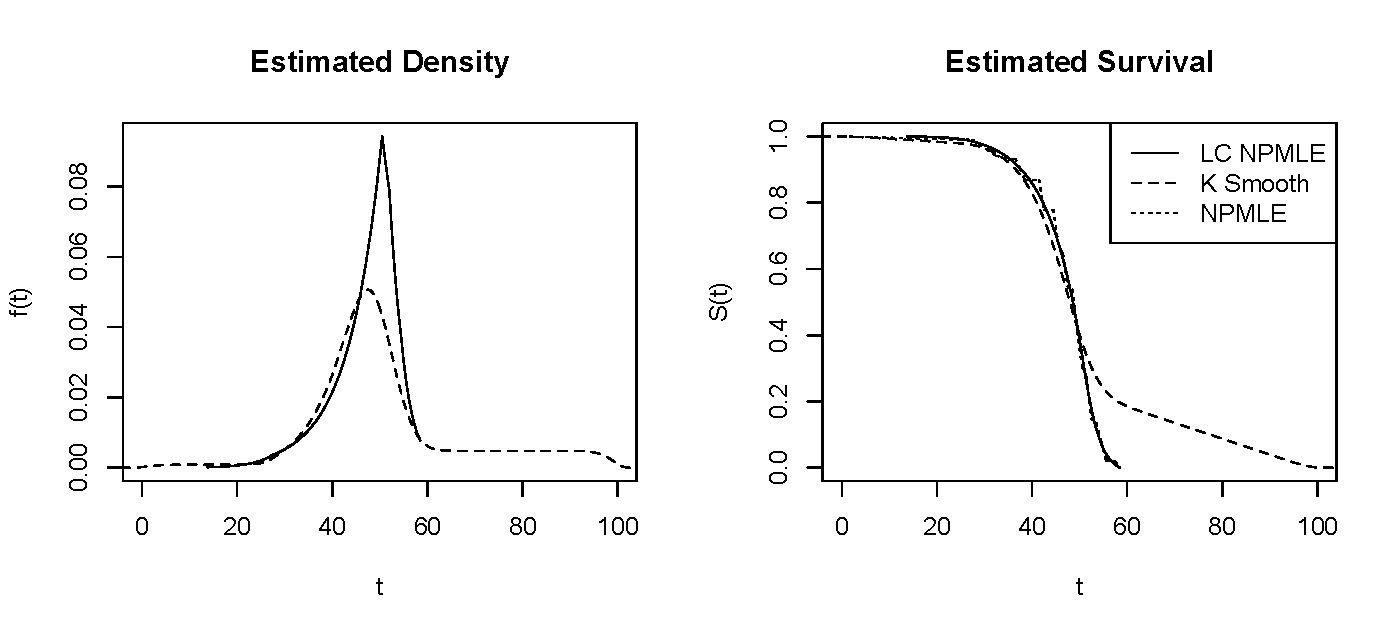
\includegraphics[width = 10cm]{FullMenoPlot.pdf}}
\caption{Estimated Functions}
\end{figure}		




	
{\section{References} }

Bagnoli, M., Bergstorm, T., (2005), Log-concave Probability and its Applications, \emph{Economic Theory} Vol 26 No. 2, 445-469

\vspace{3mm}

Betensky, R., Lindsey, J., Ryan, L., Wand, M. (1999), Local EM Estimation of the Hazard Function Interval-Censored Data, \emph{Biometrics} Vol 55 238-245

\vspace{3mm}

Braun, J., Duchense, T., Stafford, J. (2005): Local Likelihood Density Estimation for Interval Censored Data, \emph{The Canadian Journal of Statistics}, Vol 33 No.1, 39-60

\vspace{3mm}

Chang, G., Walther, G. (2007): Clustering with Mixtures of Log-Concave Distributions, \emph{Computational Statistics and Data Analysis}, Vol 51, No. 12, 6242-6251

\vspace{3mm}

D\"umbgen, L., H\"usler, A., Rufibach, K. (2011): Maximum Likelihood Estimation of a Log-Concave Density Based on Censored Data, preprint

\vspace{3mm}

D\"umbgen, L., Rufibach, K. (2009): Maximum Likelihood Estimation of a Log-Concave Density and its Distribution Function: Basic Properties and Uniform Consistency, \emph{Bernoulli}, Vol 15 No. 1 40-68

\vspace{3mm} 

Fedorov, V. (1972): \emph{Theory of Optimal Experiments}, Academic Press, 1972 

\vspace{3mm}

Gentleman, R., Geyer, C. (1994): Maximum Likelihood for Interval Censored Data: Consistency and Computation, \emph{Biometrika}, Vol 81, No. 3, 618-623

\vspace{3mm}

Gentleman, R., and Vandal, A. (2001): Computational Algorithms for Censored-Data Problems Using Intersection Graphs, \emph{Journal of Computational and Graphical Statistics}, Vol 10 No. 3, 403-421

\vspace{3mm}

Gentleman, R., and Vandal, A. (2002): Nonparametric Estimation of the Bivariate CDF for Arbitrarily Censored Data, \emph{The Canadian Journal of Statistics}, Vol 30 No. 4, 556-571

\vspace{3mm}

Grenander, U. (1956): On the Theory of Mortality Measurement. Part II, \emph{Scandinavian Actuarial Journal} Vol 39, 125-131


\vspace{3mm}

Huan, J., Wellner, J. (1997): Interval Censored Survival Data: A Review of Recent Progress, \emph{Procedings of the First Seattle Symposium in Biostatistics: Survival Analysis}, 123-169

\vspace{3mm}

Jewell, N., Laan, M., Henneman, T. (2003): Nonparametric Estimation from Current Status Data with Competing Risks, \emph{Biometrika}, Vol 90 No 1, 183-197

\vspace{3mm}

Jongbloed, G. (1998): The Iterative Convex Minorant Algorithm for Nonparametric Estimation, \emph{Journal of Computational and Graphical Statistics}, Vol 7, No. 3, 310-321

\vspace{3mm}

Krailo, M. and Pike, M. (1983): Estimation of the Distribution of Age at Natural Menopause from Prevalence Data, \emph{American Journal of Epidemiology}, Vol 117, 356-361

\vspace{3mm}

Kopperberg, C., and Stone, C. (1992): Logspline Density Estimation for Censored Data, \emph{Journal of Computational and Graphical Statistics}, Vol 1, 301-328

\vspace{3mm}

Kuhn, W., Tucker, W. (1951): Nonlinear Programming, \emph{Proceedings of 2nd Berkeley Symposium}, 481-492

\vspace{3mm}

MacMahon B. and Worcester J., (1966): Age at Menopause. United States -- 1960-1962, \emph{Nation Center for Health Statistics. Vital and Health Statistics}, Vol 11, No. 19

\vspace{3mm}

Pan, W., (2000): Smooth Estimation of the Survival Function for Interval Censored Data, \emph{Statistics in Medicine}, Vol 19, No. 19, 2611-2624

\vspace{3mm}

Rufibach, K. (2007): Computing Maximum Likelihood Estimators of a Concave Density, \emph{Journal of Statistical Computation and Simulation}, Vol 77, No. 7, 561-574

\vspace{3mm}

Treloard, A. (1981): Menstrual Cyclicity and the Pre-menopause, \emph{Maturitas}, Vol 3, 249-264

\vspace{3mm}

Turnbull, B., (1976): The Empirical Distribution Function with Arbitrarily Grouped, Censored and Truncated Data, \emph{Journal of the Royal Statistical Society. Series B (Methodological)}, Vol 38, No. 3 290-295

\vspace{3mm}

Wegman, E. (1969): A Note on Estimating a Unimodal Density, \emph{The Annals of Mathematical Statistics}, Vol 40 No. 5, 1661-1667

\vspace{3mm}


	
	 \end{document}
	